
%Este archivo no tiene contenido, mas allá de configuraciones y\o definiciones.
%todo el contenido se encuentra en los archivos secundarios que son importados por este.

\documentclass[11pt,twoside,a4paper]{extarticle}


%\\\\\\\\\\\\\\\\\\\\\\\\\\\
%Packages en uso
\usepackage{extsizes}

%Idiomas diccionario
\usepackage[english, spanish]{babel}
%\usepackage[english]{babel}

\usepackage[utf8x]{inputenc}
%\usepackage[latin1]{inputenc} 
%\usepackage[ansinew]{inputenc}
\usepackage{ucs}




%\usepackage[margin=1cm, paperwidth=21.0cm, paperheight=29.6cm]{geometry}



\usepackage[T1]{fontenc} 
\usepackage{graphicx}
\usepackage{float}
\usepackage{longtable}
%\usepackage{floatflt}
\usepackage{fancyhdr}
\usepackage{hyperref}
%\usepackage{url}
\usepackage{amsfonts}
\usepackage{amssymb}
\usepackage{textcomp}
%\usepackage[symbol]{footmisc}
%\usepackage{pst-circ}
%\usepackage{epsfig}
%\usepackage{xkeyval}
\usepackage{tabularx}
\usepackage{booktabs}


%\usepackage{color}
\usepackage[usenames,dvipsnames]{color}


%\usepackage{minted}
\usepackage{latexsym}
\usepackage{colortbl}
%\usepackage{pdfpages}
\usepackage{wrapfig}

%\usepackage{listings}
\usepackage{listingsutf8}
%\usepackage{mips}
\usepackage{appendix}
\usepackage{needspace}
\usepackage{ifplatform}
\usepackage{ifthen}



%\\\\\\\\\\\\\\\\\\\\\\\\\\\
% FOR GNUPLOT
%\usepackage{tikz}

%\usepackage[miktex]{gnuplottex}
%\usepackage{gnuplot-lua-tikz}
%\usepackage{mathpazo}
%\\\\\\\\\\\\\\\\\\\\\\\\\\\


%\\\\\\\\\\\\\\\\\\\\\\\\\\\
% FOR FIGURE CAPTION COLORS

\usepackage{caption}
\usepackage[svgnames]{xcolor}

%\\\\\\\\\\\\\\\\\\\\\\\\\\\

%\\\\\\\\\\\\\\\\\\\\\\\\\\\
% FOR FIGURE WRAPPING

\usepackage{wrapfig}

%\\\\\\\\\\\\\\\\\\\\\\\\\\\


%\\\\\\\\\\\\\\\\\\\\\\\\\\\
% FOR EQUATION CAPTION FORMAT, COLORS AND OTHERS

\usepackage{amsmath}
\usepackage{mathtools}
\usepackage{bm}
\usepackage{xcolor}
\usepackage{soul}

%\\\\\\\\\\\\\\\\\\\\\\\\\\\


%\\\\\\\\\\\\\\\\\\\\\\\\\\\
% TABLES

\usepackage{makecell, multirow, tabularx}
    \newcolumntype{L}{>{\raggedright\arraybackslash}X}
    \renewcommand\theadfont{\normalsize\bfseries\color{white}}
\usepackage{hhline}
\usepackage{setspace}

%\\\\\\\\\\\\\\\\\\\\\\\\\\\


%\\\\\\\\\\\\\\\\\\\\\\\\\\\
% UNITS

\usepackage{siunitx}

\sisetup{output-exponent-marker=\ensuremath{\mathrm{e}}}

%\\\\\\\\\\\\\\\\\\\\\\\\\\\


%\\\\\\\\\\\\\\\\\\\\\\\\\\\
% MATH

\usepackage{mathrsfs}

\usepackage{mathtools}

\usepackage{amsmath,mleftright}

\usepackage{xparse}

\numberwithin{equation}{subsection}

\NewDocumentCommand{\evalat}{sO{\big}mm}{%
  \IfBooleanTF{#1}
   {\mleft. #3 \mright|_{#4}}
   {#3#2|_{#4}}%
}

\newcommand{\mathcolorbox}[2]{\colorbox{#1}{$\displaystyle #2$}}

%\\\\\\\\\\\\\\\\\\\\\\\\\\\

%\\\\\\\\\\\\\\\\\\\\\\\\\\\
%!!!!!!!!!!!!!!!!!!!!!!!!! DETECCION DE PLATAFORMA !!!!!!!!!!!!!!!!!!!!!!!!!!!!!!!!!
%Permite que sea compilado tanto en windows como en *IX sin cambio alguno.
\newboolean{IsWindows}
\ifwindows
\setboolean{IsWindows}{true}
\else
\setboolean{IsWindows}{false}
\fi
%\\\\\\\\\\\\\\\\\\\\\\\\\\\
%!!!!!!!!!!!!!!!!!!!!!!!!!!!!!!!!!!!!!!!!!!!!!!!!!!!!!!!!!!!!!!!!!!!!!!!!!!!!!!!!!!!!

%\\\\\\\\\\\\\\\\\\\\\\\\\\\
%Idiomas
\hyphenrules{spanish}
%\\\\\\\\\\\\\\\\\\\\\\\\\\\

%\\\\\\\\\\\\\\\\\\\\\\\\\\\
%3D
%\usepackage{media9}
%\\\\\\\\\\\\\\\\\\\\\\\\\\\


%\\\\\\\\\\\\\\\\\\\\\\\\\\\
%Comandos personalizados

\newcommand{\titulo}{Monografía final de la materia}
\newcommand{\titulolargo}{Introducción a la tecnología FTTH}
\newcommand{\materia}{Video y Redes de Cable - 66.81}
\newcommand{\fiuba}{Facultad de Ingeniería - UBA}
\newcommand{\cuatrimestre}{2\sptext{do} cuat. 2020} %\sptext{do} $2^{do}$

 
\newcommand{\autorA}{\textsc{Luna} Diego}
\newcommand{\padronA}{75451}
\newcommand{\mailA}{\weblink{mailto:diegorluna@gmail.com}{diegorluna@gmail.com}}
   
 
 
\newcommand{\docenteA}{Ing. \textsc{GROSSI} Cayetano Roberto}
\newcommand{\docenteB}{Ing. \textsc{ALVAREZ} Guillermo}



\newcommand{\thedate}{1 de Marzo de 2021}


\newcommand{\HRule}{\rule{\linewidth}{0.3mm}}

%\\\\\\\\\\\\\\\\\\\\\\\\\\\


%\\\\\\\\\\\\\\\\\\\\\\\\\\\
%Título,  autor del documento y fecha
\title{\titulo}
\author{\autorA}
\date{\thedate}
%\\\\\\\\\\\\\\\\\\\\\\\\\\\


%\\\\\\\\\\\\\\\\\\\\\\\\\\\
\setcounter{secnumdepth}{5}
\setcounter{tocdepth}{5}
%\\\\\\\\\\\\\\\\\\\\\\\\\\\


%\\\\\\\\\\\\\\\\\\\\\\\\\\\
%suppress widows and orphans
\widowpenalty=9999
\clubpenalty=9999
%\\\\\\\\\\\\\\\\\\\\\\\\\\\


%\\\\\\\\\\\\\\\\\\\\\\\\\\\
%equation numbers to subsection level
%\numberwithin{equation}{subsection}
%\numberwithin{equation}{section}
%\\\\\\\\\\\\\\\\\\\\\\\\\\\


%\\\\\\\\\\\\\\\\\\\\\\\\\\\
%equation numbers to subsection level
%\numberwithin{table}{subsection}
\numberwithin{table}{subsection}
%\\\\\\\\\\\\\\\\\\\\\\\\\\\



%\\\\\\\\\\\\\\\\\\\\\\\\\\\
%figure numbers to subsection level
%\renewcommand{\thefigure}{\thesubsection.\arabic{figure}}
\renewcommand{\thefigure}{\thesection.\arabic{figure}}
%\\\\\\\\\\\\\\\\\\\\\\\\\\\

%\setlength{\arrayrulewidth}{0.6pt}


%\\\\\\\\\\\\\\\\\\\\\\\\\\\
\newcolumntype{z}[1]{%
>{\centering\hspace{0pt}}p{#1}}%

\newcolumntype{y}[1]{%
>{\raggedleft\hspace{0pt}}p{#1}}% 

\newcolumntype{x}[1]{%
>{\raggedright\hspace{0pt}}p{#1}}% 

\newcolumntype{w}[1]{%
>{\centering\hspace{0pt}}m{#1}}%

\newcolumntype{v}[1]{%
>{\raggedleft\hspace{0pt}}m{#1}}% 

\newcolumntype{u}[1]{%
>{\raggedright\hspace{0pt}}m{#1}}% 


\newcommand{\tn}{\tabularnewline}
%\\\\\\\\\\\\\\\\\\\\\\\\\\\




%\\\\\\\\\\\\\\\\\\\\\\\\\\\
% Generales
\newcommand{\quotemarks}[1]{``#1''}
\newcommand{\simplequotemarks}[1]{`#1'}
%\\\\\\\\\\\\\\\\\\\\\\\\\\\


%\\\\\\\\\\\\\\\\\\\\\\\\\\\
% Símbolos de las unidades

%\newcommand{\volt}[1]{\mbox{#1 V}}
%\newcommand{\milivolt}[1]{\mbox{#1 mV}}
%\newcommand{\hertz}[1]{\mbox{#1 Hz}}
%\newcommand{\kilohertz}[1]{\mbox{#1 kHz}}
%\newcommand{\megahertz}[1]{\mbox{#1 MHz}}
%\newcommand{\farad}[1]{\mbox{#1 F}}
%\newcommand{\nanofarad}[1]{\mbox{#1 nF}}
%\newcommand{\microfarad}[1]{\mbox{#1 $\mu$F}}
%\newcommand{\picofarad}[1]{\mbox{#1 pF}}
%\newcommand{\fentofarad}[1]{\mbox{#1 fF}}
%\newcommand{\ohm}[1]{\mbox{#1 $\Omega$}}
%\newcommand{\miliohm}[1]{\mbox{#1 m$\Omega$}}
%\newcommand{\kiloohm}[1]{\mbox{#1 k$\Omega$}}
%\newcommand{\megaohm}[1]{\mbox{#1 M$\Omega$}}
%\newcommand{\amper}[1]{\mbox{#1 A}}
%\newcommand{\miliamper}[1]{\mbox{#1 mA}}
%\newcommand{\microamper}[1]{\mbox{#1 $\mu$A}}
%\newcommand{\picoamper}[1]{\mbox{#1 pA}}
%\newcommand{\fentoamper}[1]{\mbox{#1 fA}}
%\newcommand{\s}[1]{\mbox{#1 s}}
%\newcommand{\milis}[1]{\mbox{#1 ms}}
%\newcommand{\micros}[1]{\mbox{#1 $\mu$s}}
%\newcommand{\nanos}[1]{\mbox{#1 ns}}
%\newcommand{\miliamperporvolt}[1]{ \mbox{#1 $\frac{mA}{V}$}}
%\newcommand{\miliamperporvoltcuad}[1]{ \mbox{#1 $\frac{mA}{V^2}$}}
%\newcommand{\decibel}[1]{\mbox{#1 dB}}
%\newcommand{\decibeli}[1]{\mbox{#1 dBi}}


% Nombres de las unidades
%\newcommand{\Metro}{\mbox{metro}}
%\newcommand{\Volt}{\mbox{Volt}}
%\newcommand{\Amper}{\mbox{Ampere}}
%\newcommand{\Farad}{\mbox{Farad}}

\newcommand{\spice}{\mbox{\textit{\textbf{SPICE}}}}
\newcommand{\schematic}{\mbox{\textit{\textbf{SCHEMATIC}}}}

\newcommand{\parallelresistors}{\mathbin{\!/\mkern-5mu/\!}}


%\\\\\\\\\\\\\\\\\\\\\\\\\\\

%\\\\\\\\\\\\\\\\\\\\\\\\\\\
% Dispositivos

\newcommand{\mosfet}{\mbox{\textbf{MOSFET}}}
\newcommand{\nmosfet}{\mbox{\textbf{NMOSFET}}}
\newcommand{\bjtnpn}{\mbox{\textbf{BJT NPN}}}
\newcommand{\bjtpnp}{\mbox{\textbf{BJT PNP}}}

%\\\\\\\\\\\\\\\\\\\\\\\\\\\

%\\\\\\\\\\\\\\\\\\\\\\\\\\\
% Plataformas

\newcommand{\platformhost}{\textbf{x86(\_64)\textbackslash Linux}}
\newcommand{\platformguest}{\textbf{pmax\textbackslash NetBSD}}

\newcommand{\oshost}{\textbf{Linux}}
\newcommand{\osguest}{\textbf{NetBSD}}

\newcommand{\MIPS}{\textbf{MIPS32}}
%\\\\\\\\\\\\\\\\\\\\\\\\\\\


%\\\\\\\\\\\\\\\\\\\\\\\\\\\
% Programación

\newcommand{\GNU}{\textbf{GNU}}

\newcommand{\GCC}{\textbf{GCC}}

\newcommand{\GDB}{\textbf{GDB}}

\newcommand{\GXEMUL}{\textbf{GXemul}}

\newcommand{\langc}{\textbf{\quotemarks{C}}}

\newcommand{\langass}{\textbf{assembly}}

\newcommand{\langmipsass}{\textbf{MIPS32 assembly}}

\newcommand{\make}{\textbf{make}}
%\\\\\\\\\\\\\\\\\\\\\\\\\\\


%\\\\\\\\\\\\\\\\\\\\\\\\\\\
% Archivos

\newcommand{\quotefile}[1]{\textit{\quotemarks{#1}}}

\newcommand{\filebox}[2]{%

\begin{tabular}{l}

\multicolumn{1}{>{\columncolor{#2}}l}{#1} 
	
\end{tabular}

}%
%\\\\\\\\\\\\\\\\\\\\\\\\\\\



%\\\\\\\\\\\\\\\\\\\\\\\\\\\
% Math
\newcommand{\Reales}{\mathbb{R}}
\newcommand{\Complejos}{\mathbb{C}}
\newcommand{\numnorm}[1]{\left|#1\right|}
\newcommand{\vectornorm}[1]{\left|\left|#1\right|\right|}
%\\\\\\\\\\\\\\\\\\\\\\\\\\\


%\\\\\\\\\\\\\\\\\\\\\\\\\\\
% Counters
\newcommand{\resetallcounters}{%
\setcounter{figure}{0}
\setcounter{equation}{0}
\setcounter{table}{0}
}%
%\\\\\\\\\\\\\\\\\\\\\\\\\\\



%\\\\\\\\\\\\\\\\\\\\\\\\\\\
% Definiciones de colores.
\definecolor{Deepblue}{rgb}{0.00,0.00,0.70}
\definecolor{Deepgreen}{rgb}{0.09,0.45,0.20}
\definecolor{Darkgreen}{RGB}{0, 128, 0}
\definecolor{Purple}{rgb}{1,0,1}
\definecolor{Deeppurple}{rgb}{0.2,0,1}
\definecolor{Gray}{rgb}{0.3,0.3,0.3}
\definecolor{Lightblue}{rgb}{0.60, 0.80, 1.00}
\definecolor{Lightyellow}{rgb}{1.00,1.00,0.60}
\definecolor{LightButter}{rgb}{0.98,0.91,0.31}
\definecolor{LightOrange}{rgb}{0.98,0.68,0.24}
\definecolor{LightChocolate}{rgb}{0.91,0.72,0.43}
\definecolor{LightChameleon}{rgb}{0.54,0.88,0.20}
\definecolor{LightSkyBlue}{rgb}{0.45,0.62,0.81}
\definecolor{LightPlum}{rgb}{0.68,0.50,0.66}
\definecolor{LightScarletRed}{rgb}{0.93,0.16,0.16}
\definecolor{Butter}{rgb}{0.93,0.86,0.25}
\definecolor{Orange}{rgb}{0.96,0.47,0.00}
\definecolor{Chocolate}{rgb}{0.75,0.49,0.07}
\definecolor{Chameleon}{rgb}{0.45,0.82,0.09}
\definecolor{SkyBlue}{rgb}{0.20,0.39,0.64}
\definecolor{Plum}{rgb}{0.46,0.31,0.48}
\definecolor{ScarletRed}{rgb}{0.80,0.00,0.00}
\definecolor{DarkButter}{rgb}{0.77,0.62,0.00}
\definecolor{DarkOrange}{rgb}{0.80,0.36,0.00}
\definecolor{DarkChocolate}{rgb}{0.56,0.35,0.01}
\definecolor{DarkChameleon}{rgb}{0.30,0.60,0.02}
\definecolor{DarkSkyBlue}{rgb}{0.12,0.29,0.53}
\definecolor{DarkPlum}{rgb}{0.36,0.21,0.40}
\definecolor{DarkScarletRed}{rgb}{0.64,0.00,0.00}
\definecolor{Aluminium1}{rgb}{0.93,0.93,0.92}
\definecolor{Aluminium2}{rgb}{0.82,0.84,0.81}
\definecolor{Aluminium3}{rgb}{0.73,0.74,0.71}
\definecolor{Aluminium4}{rgb}{0.53,0.54,0.52}
\definecolor{Aluminium5}{rgb}{0.33,0.34,0.32}
\definecolor{Aluminium6}{rgb}{0.18,0.20,0.21}

\definecolor{EQColor}{RGB}{50,205,50}
\definecolor{FIGColor}{RGB}{255,155,0}
\definecolor{TABLEColor}{RGB}{00,255,255}



\definecolor{APENDLINKColor}{rgb}{0.96,0.47,0.00}
\definecolor{SECTLINKColor}{rgb}{1.00,0.30,0.00}
\definecolor{FILELINKColor}{rgb}{1.00,0.00,0.00}
\definecolor{INTERNALLINKColor}{rgb}{1.00,0.00,0.00}
\definecolor{WEBLINKColor}{rgb}{0.00,0.00,1.00}
\definecolor{CITELINKColor}{RGB}{141,199,126}
\definecolor{TABLELINKColor}{RGB}{199,199,0}


%\definecolor{EQColor}{rgb}{0.00,0.36,0.80}
%\definecolor{FIGColor}{cmyk}{1,0.00,0.00,0.00}
%\definecolor{TABLEColor}{RGB}{0,199,25}



%\definecolor{APENDLINKColor}{rgb}{0.10,0.47,0.00}
%\definecolor{SECTLINKColor}{rgb}{0.00,0.00,1.00}
%\definecolor{FILELINKColor}{rgb}{0.00,0.00,1.00}
%\definecolor{INTERNALLINKColor}{rgb}{0.00,0.00,1.00}
%\definecolor{WEBLINKColor}{rgb}{0.00,0.00,1.00}
%\definecolor{CITELINKColor}{RGB}{141,199,126}
%\definecolor{TABLELINKColor}{RGB}{199,199,0}


\definecolor{HeadersColor}{RGB}{0,137,182}

%\\\\\\\\\\\\\\\\\\\\\\\\\\\


%\\\\\\\\\\\\\\\\\\\\\\\\\\\
% FOR FIGURE CAPTION COLORS

\DeclareCaptionFont{FIGFont}{\color{FIGColor}}
\captionsetup[figure]{labelfont={FIGFont,bf}}

\newcommand{\figref}[1]{\textcolor{FIGColor}{[\ref{#1}]}}
%\\\\\\\\\\\\\\\\\\\\\\\\\\\


%\\\\\\\\\\\\\\\\\\\\\\\\\\\
% FOR TABLE CAPTION COLORS

\DeclareCaptionFont{TABLEFont}{\color{TABLEColor}}
\captionsetup[table]{labelfont={TABLEFont,bf}}

\newcommand{\tableref}[1]{\textcolor{TABLEColor}{[\ref{#1}]}}


%\captionsetup[table]{style=fortables}
%\captionsetup[figure]{style=forfigures}
%\\\\\\\\\\\\\\\\\\\\\\\\\\\


%\\\\\\\\\\\\\\\\\\\\\\\\\\\
% FOR EQUATION CAPTION FORMAT, COLORS AND OTHERS

\newtagform{brackets2}[\textcolor{EQColor}]{\textcolor{EQColor}(}{\textcolor{EQColor})}
\usetagform{brackets2}

%\\\\\\\\\\\\\\\\\\\\\\\\\\\


%\\\\\\\\\\\\\\\\\\\\\\\\\\\
% FOR EQUATION CAPTION COLORS
%\makeatletter %% Without ams
%\def\@eqnnum{{\normalfont\normalcolor[\theequation]}}
%\makeatother

%But amsmath redefines the numbering of equations, so then you can do:

%\makeatletter %% With ams
%\def\tagform@#1{\maketag@@@{[\ignorespaces#1\unskip\@@italiccorr]}}
%\makeatother 
%\\\\\\\\\\\\\\\\\\\\\\\\\\\


%\\\\\\\\\\\\\\\\\\\\\\\\\\\
% FOR APENDIX REFERENCE

\newcommand{\apendref}[1]{\textcolor{APENDLINKColor}{[\ref{#1}]}}

%\\\\\\\\\\\\\\\\\\\\\\\\\\\


%\\\\\\\\\\\\\\\\\\\\\\\\\\\
% FOR SECTION REFERENCE

\newcommand{\sectref}[1]{\textcolor{SECTLINKColor}{[\ref{#1}]}}

%\\\\\\\\\\\\\\\\\\\\\\\\\\\


%\\\\\\\\\\\\\\\\\\\\\\\\\\\
% WEB LINK

\newcommand{\weblink}[2]{\href{#1}{\textcolor{WEBLINKColor}{#2}}}

%\\\\\\\\\\\\\\\\\\\\\\\\\\\


%\\\\\\\\\\\\\\\\\\\\\\\\\\\
% FILE LINK

\newcommand{\filelink}[2]{\href{#1}{\textcolor{FILELINKColor}{#2}}}

%\\\\\\\\\\\\\\\\\\\\\\\\\\\


%\\\\\\\\\\\\\\\\\\\\\\\\\\\
% CITE LINK
\newcommand{\citelink}[1]{\textcolor{LimeGreen}{\cite{#1}}}

%\\\\\\\\\\\\\\\\\\\\\\\\\\\


\hypersetup{
%	bookmarksnumbered,
%	pdfpagemode={UseOutlines},
%    bookmarks=true,         				% show bookmarks bar?
    unicode=true,          					% non-Latin characters in Acrobat’s bookmarks
    pdftoolbar=true,        				% show Acrobat’s toolbar?
    pdfmenubar=true,        				% show Acrobat’s menu?
%    pdffitwindow=false,    				% window fit to page when opened
%    pdfstartview={FitH},   				% fits the width of the page to the window
    pdftitle={\titulo},   					% title
    pdfauthor={\autorA},    				% author
    pdfsubject={\materia},   				% subject of the document
%    pdfcreator={\LaTeX},   				% creator of the document
%    pdfproducer={Producer},				% producer of the document
    pdfkeywords={TL} {TP}, 					% list of keywords
    pdfnewwindow=true,      				% links in new window
    linktoc=all,							%
    colorlinks=false,  						% false: boxed links; true: colored links	
	linkcolor=INTERNALLINKColor,			% color of internal links
    citecolor=CITELINKColor,    			% color of links to bibliography
    filecolor=FILELINKColor,   	 			% color of file links
    urlcolor=WEBLINKColor,       			% color of external links	
	linkbordercolor=INTERNALLINKColor,		% color of internal links
	citebordercolor=CITELINKColor,			% color of links to bibliography
    filebordercolor=FILELINKColor,    		% color of file links
    urlbordercolor=WEBLINKColor}	       	% color of external links	    
   				
	


%\\\\\\\\\\\\\\\\\\\\\\\\\\\
%Comportamiento de los links a archivos externos.
%\hypersetup{pdfnewwindow=true}
%\\\\\\\\\\\\\\\\\\\\\\\\\\\

%\\\\\\\\\\\\\\\\\\\\\\\\\\\
%Tamaños de la página y margenes

\linespread{1.3}
\oddsidemargin .1cm
\evensidemargin .1cm
\textwidth 16.5cm
\topmargin 0in
\voffset = 0pt
\textheight 21.08cm %8.3in
%\\\\\\\\\\\\\\\\\\\\\\\\\\\



%\pagestyle{fancy}


%\\\\\\\\\\\\\\\\\\\\\\\\\\\
%Encabezado y pie de páginas para todas las páginas normales

\fancypagestyle{allpages}{%

\fancyhf{}  

\renewcommand{\headrulewidth}{0.4pt}
\renewcommand{\footrulewidth}{0.4pt}

%No convierte a mayúscula los nombres de capítulo y sección 
%ni muestra el número.
%\renewcommand{\chaptermark}[1]{}
\renewcommand{\sectionmark}[1]{\markright{##1}{}}
\renewcommand{\subsectionmark}[1]{}
\renewcommand{\subsubsectionmark}[1]{}


\setlength{\headheight}{12pt}

   
%\fancyhf[LOH,REH]{\fiuba}
%\fancyhf[ROH,LEH]{\titulo}

\fancyhf[LH]{
\includegraphics[width=3cm]{./img/logo_encabezado_fiuba}}
\fancyhf[CH]{\small{\materia}}
\fancyhf[RH]{\titulo} 

\fancyhf[LOF,REF]{\small{\cuatrimestre}}
\fancyhf[CF]{\small{\rightmark}}
\fancyhf[LEF, ROF]{\textbf{\thepage}} 

}

%\\\\\\\\\\\\\\\\\\\\\\\\\\\


%\\\\\\\\\\\\\\\\\\\\\\\\\\\
%Encabezado y pie de páginas para el índice
\fancypagestyle{indexstyle}{%

\fancyhf{} % clear all header and footer fields

\renewcommand{\headrulewidth}{0.4pt}
\renewcommand{\footrulewidth}{0.4pt}

\setlength{\headheight}{12pt}


\fancyhf[LH]{
\includegraphics[width=3cm]{./img/logo_encabezado_fiuba}}
\fancyhf[CH]{\small{\materia}}
\fancyhf[RH]{\titulo}

\fancyhf[LOF,REF]{\small{\cuatrimestre}}
\fancyhf[CF]{\small{Índice}}
\fancyhf[LEF, ROF]{\textbf{\thepage}} 

%\color{red}

}
%\\\\\\\\\\\\\\\\\\\\\\\\\\\




%\\\\\\\\\\\\\\\\\\\\\\\\\\\
%Encabezado y pie de páginas para el código
\fancypagestyle{codestyle}{%

\fancyhf{} % clear all header and footer fields

\renewcommand{\headrulewidth}{0.4pt}
\renewcommand{\footrulewidth}{0.4pt}

%No convierte a mayúscula los nombres de capítulo y sección 
%ni muestra el número.
%\renewcommand{\chaptermark}[1]{}
\renewcommand{\sectionmark}[1]{}
\renewcommand{\subsectionmark}[1]{}
\renewcommand{\subsubsectionmark}[1]{\markright{##1}}

\setlength{\headheight}{12pt}

\fancyhf[LH]{\small{\fiuba}}
\fancyhf[CH]{\small{\materia}}
\fancyhf[RH]{\titulo}
\fancyhf[LOF,REF]{\small{\cuatrimestre}}
\fancyhf[CF]{\small{Archivo: \color{DarkBlue}\rightmark}}
%\bfseries{\color{red} \filename
\fancyhf[LEF, ROF]{\textbf{\thepage}} 


\normalfont
}
%\\\\\\\\\\\\\\\\\\\\\\\\\\\



\newcommand{\themark}{}

%\\\\\\\\\\\\\\\\\\\\\\\\\\\
%Encabezado y pie de páginas para el código
\fancypagestyle{codeconsstyle}{%

\fancyhf{} % clear all header and footer fields

\renewcommand{\headrulewidth}{0.4pt}
\renewcommand{\footrulewidth}{0.4pt}


\setlength{\headheight}{12pt}


\fancyhf[LH]{\small{\fiuba}}
\fancyhf[CH]{\small{\materia}}
\fancyhf[RH]{\titulo}

\fancyhf[LOF,REF]{\small{\cuatrimestre}}
\fancyhf[CF]{\small{\themark}}
\fancyhf[LEF, ROF]{\textbf{\thepage}} 

}
%\\\\\\\\\\\\\\\\\\\\\\\\\\\




%\\\\\\\\\\\\\\\\\\\\\\\\\\\
%Encabezado y pie de páginas para el índice
\fancypagestyle{bibliostyle}{%

\fancyhf{} % clear all header and footer fields

\renewcommand{\headrulewidth}{0.4pt}
\renewcommand{\footrulewidth}{0.4pt}

\setlength{\headheight}{12pt}


\fancyhf[LH]{\small{\fiuba}}
\fancyhf[CH]{\small{\materia}}
\fancyhf[RH]{\titulo}

\fancyhf[LOF,REF]{\small{\cuatrimestre}}
\fancyhf[CF]{\small{Bibliografía}}
\fancyhf[LEF, ROF]{\textbf{\thepage}} 

}
%\\\\\\\\\\\\\\\\\\\\\\\\\\\



%\\\\\\\\\\\\\\\\\\\\\\\\\\\
%Renuevo los nombres de los apéndices.
\renewcommand{\appendixpagename}{Apéndices}
\renewcommand{\appendixtocname}{Apéndices}
%\\\\\\\\\\\\\\\\\\\\\\\\\\\

%\\\\\\\\\\\\\\\\\\\\\\\\\\\
%Renuevo el símbolo de los items.
\renewcommand\labelitemi{$\bullet$}
%\\\\\\\\\\\\\\\\\\\\\\\\\\\




%\\\\\\\\\\\\\\\\\\\\\\\\\\\\\\\


%\\\\\\\\\\\\\\\\\\\\\\\\\\\\\\\

%-------------------------------------------------
%--------------- BEGIN DOCUMENT ------------------
%-------------------------------------------------
\begin{document}



%\\\\\\\\\\\\\\\\\\\\\\\\\\\
%Incluyo la caratula
%Caratula
\begin{titlepage}
%
% Sin cabecera ni pie de página:
%


\thispagestyle{empty}


 %Título:

	\begin{center}
	
	\textcolor[RGB]{0,0,0}{\rule{\linewidth}{2pt}}
	
   	\begin{figure}[H]
    		\centering
    		
\includegraphics[width=0.7 \textwidth]{./img/fiuba}
  	\end{figure}




		\vspace{1.2cm}


		\textsc{\huge \materia}\\
		\vspace{0.45cm}
		\Huge{\titulo}\\
		\HRule \\
		\vspace{0.15cm}
		\Large{\textbf{\titulolargo}}\\
		\HRule \\
		\vspace{0.15cm}



		\begin{flushleft}
			\begin{tabularx}{\textwidth}{@{\extracolsep{\fill}} ll|l}
				\emph{Alumnos:}&&\emph{Docentes:} \\
				\autorA & Padrón N\textdegree \space \padronA & \docenteA \\
				\mailA  &  & \docenteB \\
				&  & \\
				&  & \\				
				&  & \\
				&  & \\	

%% \begin{normalsize}\textbf{(\textbf{*}) Docente asignado.}\end{normalsize}\\				        				
			\end{tabularx}
		\end{flushleft}


		\vfill
%        \vspace{0.1cm}
		% Bottom of the page
		{\Large \thedate}

	\textcolor[RGB]{0,0,0}{\rule{\linewidth}{2pt}}

	\end{center}


\end{titlepage}














\thispagestyle{empty}
\cleardoublepage
%\\\\\\\\\\\\\\\\\\\\\\\\\\\
	
%\\\\\\\\\\\\\\\\\\\\\\\\\\\
%Reinicio la cuenta y seteo el estilo de headers y footers.
\pagestyle{indexstyle}
\pagenumbering{Roman}
\setcounter{page}{1}
%\\\\\\\\\\\\\\\\\\\\\\\\\\\

%\\\\\\\\\\\\\\\\\\\\\\\\\\\
\begin{small}
\tableofcontents 
\addcontentsline{toc}{section}{Índice}
%\phantomsection\pdfbookmark[0]{\indexname}{bookmarkForTheIndex}

\clearpage

\listoffigures

\clearpage

\listoftables

\end{small}

\cleardoublepage
%\\\\\\\\\\\\\\\\\\\\\\\\\\\

%\\\\\\\\\\\\\\\\\\\\\\\\\\\
%Reinicio la cuenta y seteo el stilo de headers y footers.
\pagestyle{allpages}
\setcounter{page}{1}
\pagenumbering{arabic}
%\\\\\\\\\\\\\\\\\\\\\\\\\\\


%\\\\\\\\\\\\\\\\\\\\\\\\\\\
\section{Introducción}
\resetallcounters

\fontsize{13}{14}\selectfont


La fibra óptica monomodo, con su ancho de banda prácticamente ilimitado, es actualmente el medio de transmisión preferido en las redes de telecomunicación, de transporte y metropolitanas. La utilización de cable de fibra óptica (en lugar de cable de cobre) reduce significativamente los costes del equipo y de mantenimiento, a la vez que aumenta drásticamente la calidad del servicio (QoS); y, ahora más que nunca, muchos clientes corporativos tienen acceso a servicios de fibra óptica de punto a punto (P2P).

Los cables de fibra óptica se implantan ahora en la última milla: el segmento de la red que va desde la oficina central (CO) al abonado. Dado que, hasta hace poco, ese segmento se basaba normalmente en el cobre, los servicios de alta velocidad disponibles para los clientes residenciales y las empresas pequeñas se limitaban a líneas de abonados digitales genéricas (xDSL) y transmisiones coaxiales de fibra híbridas (HFC). La principal alternativa (transmisión inalámbrica con servicio de retransmisión directa (DBS)) requiere una antena y un transceptor. Por tanto, en el contexto actual, con su enorme demanda de ancho de banda y de servicios de mayor velocidad a distancias mayores, el transporte basado en cobre e inalámbrico presenta las siguientes carencias:
      

\begin{itemize}
\item Ancho de banda limitado.
\item Diferentes medios y equipos que requieren un mantenimiento específico.
\end{itemize}


Pese a que los cables de fibra óptica superan todas esas limitaciones, uno de los obstáculos en la provisión de servicios de fibra óptica directamente a los hogares y a las pequeñas empresas ha sido el elevado coste de conectar a cada abonado a la CO.

Para superar los problemas de costes, actores importantes de la industria crearon la organización de normalización Red de Acceso de Servicio Completo (Full-Service Access Network, FSAN), fundada para facilitar el desarrollo de especificaciones adecuadas de sistemas de equipos de redes de acceso.

La Unión Internacional de Telecomunicaciones (ITU-T) convirtió las especificaciones FSAN en recomendaciones. La especificación FSAN para redes ópticas pasivas (PONs) basadas en ATM se convirtió en una norma internacional en 1998 y fue adoptada por la ITU como recomendación G.983.1.


\clearpage
%\\\\\\\\\\\\\\\\\\\\\\\\\\\


%\\\\\\\\\\\\\\\\\\\\\\\\\\\
 \section{Tecnologías utilizadas en FTTH}
 \resetallcounters
 Nuevas normas como, por ejemplo, las establecidas por la ITU-T, el IEC y el Instituto de Ingeniería Electrónica y Eléctrica (IEEE), han incrementado en gran medida la estandarización del diseño, la viabilidad y la seguridad de PONs; lo que brinda la oportunidad de economías escala y menores costes, no concebibles anteriormente.

Las figuras~\figref{fig:PON_Now}~y~\figref{fig:PON_Next} resumen los principales parámetros que definen esas normas.

\begin{figure}[H]
	\centering
	\includegraphics[width=0.75\textwidth]{./img/punto1/Tecnologías-PON-actualmente-implantadas.jpg}
	\caption{Tecnologías PON actualmente implantadas}
	\label{fig:PON_Now}
\end{figure}


\begin{figure}[H]
	\centering
	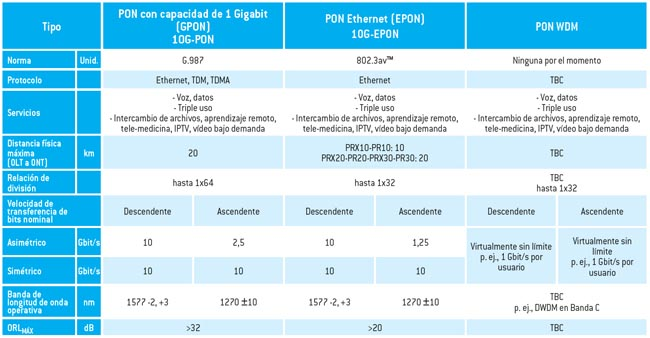
\includegraphics[width=0.75\textwidth]{./img/punto1/Tecnologías-PON-de-próxima-generación.jpg}
	\caption{Tecnologías PON de próxima generación}
	\label{fig:PON_Next}
\end{figure}
 \clearpage
%\\\\\\\\\\\\\\\\\\\\\\\\\\\

%\\\\\\\\\\\\\\\\\\\\\\\\\\\
 \section{Arquitecturas FTTH}
 \resetallcounters
 La figura~\figref{fig:FTTH_general} muestra la arquitectura general de una red FTTH típica. En la CO (también denominada cabecera), la red de telefonía pública conmutada (PSTN) y los servicios de Internet se interconectan con la red de distribución óptica (ODN) mediante el terminal de línea óptica (OLT). Las longitudes de onda descendentes de 1490 nm y ascendentes de 1310 nm se utilizan para transmitir datos y voz. Los servicios de vídeo RF analógicos se convierten en formato óptico a la longitud de onda 1550 nm mediante el transmisor de vídeo óptico. Las longitudes de onda de 1550 nm y 1490 nm son combinadas por el acoplador WDM y se transmiten juntas de forma descendente. IPTV se transmite sobre 1490 nm.



\begin{wrapfigure}[12]{l}{0.55\textwidth}
  \begin{center}
   	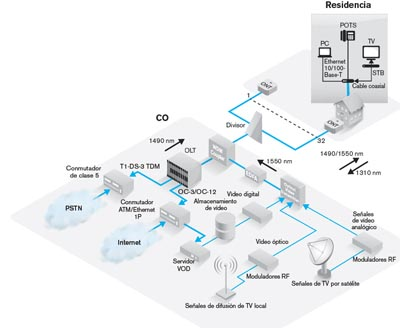
\includegraphics[width=0.55\textwidth]{./img/punto2/Arquitectura-FTTH-general.jpg}	
   	\caption{Arquitectura FTTH general}
	\label{fig:FTTH_general}
  \end{center}  
\end{wrapfigure}


En resumen, las tres longitudes de onda (1310, 1490 y 1550 nm) transportan simultáneamente diferente información y en varias direcciones sobre la misma fibra. El cable de entrada F1 transporta las señales ópticas entre la CO y el divisor, lo cual permite conectar varios ONT a la misma fibra de entrada. Se requiere un ONT para cada abonado y proporciona conexiones para los distintos servicios (voz, datos y vídeo).\\ \\


\vspace{1cm}


Dado que un OLT presta servicio hasta un número de 32 abonados (más de 64 con GPON), normalmente se necesitan muchos OLTs que salgan de la misma CO para servir a una comunidad. Hay diferentes arquitecturas para conectar abonados a la PON. La más sencilla utiliza un divisor único (véase la figura~\figref{fig:Arq_one_layer}), pero también pueden emplearse varios divisores (véase la figura~\figref{fig:Arq_two_layers}).


\begin{figure}[H]
	\centering
	\includegraphics[width=0.80\textwidth]{./img/punto2/Arquitectura-de-etapa-única.jpg}
	\caption{Arquitectura de etapa única}
	\label{fig:Arq_one_layer}
\end{figure}



\begin{figure}[H]
	\centering
	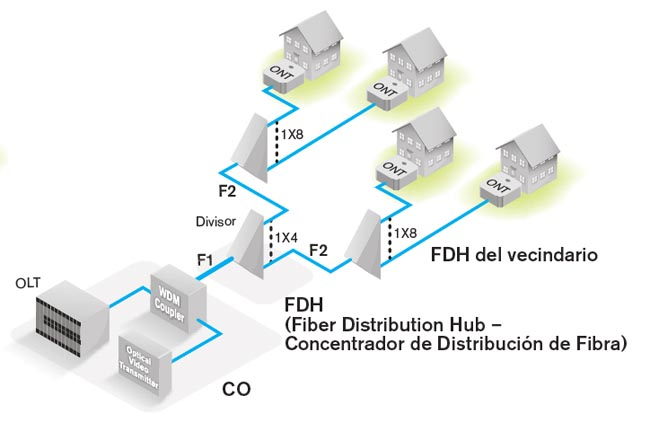
\includegraphics[width=0.80\textwidth]{./img/punto2/Arquitectura-de-dos-etapas.jpg}
	\caption{Arquitectura de dos etapas}
	\label{fig:Arq_two_layers}
\end{figure}






 \clearpage
%\\\\\\\\\\\\\\\\\\\\\\\\\\\

%\\\\\\\\\\\\\\\\\\\\\\\\\\\
 \section{Equipo de red para distribución óptica pasiva}
 \resetallcounters
 El equipo de red de distribución óptica pasiva (ODN) consiste en un equipo y componentes ubicados entre el OLT (activo) y las instalaciones del cliente (el ONT; activo); este incluye componentes tanto ópticos como no ópticos de la red. Los componentes ópticos forma la red de distribución óptica (ODN) e incluyen empalmes (fusión y mecánicos), conectores, divisores, acopladores WDM, cables de fibra óptica, cordones de conexión y posiblemente terminales de acceso con cables de acceso. Los componentes no ópticos incluyen pedestales, armarios, paneles de conexiones, cajas de empalme y hardware diverso (véase la figura~\figref{fig:ODN_passive}).


\begin{figure}[H]
	\centering
	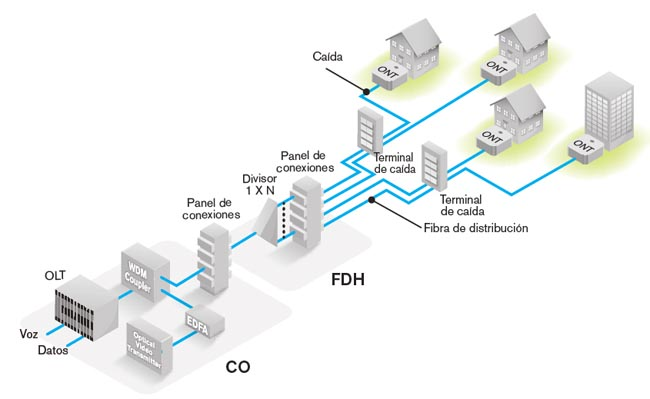
\includegraphics[width=0.75\textwidth]{./img/punto3/Equipo-ODN-pasivo.jpg}
	\caption{Equipo ODN pasivo}
	\label{fig:ODN_passive}
\end{figure}
 \clearpage
%\\\\\\\\\\\\\\\\\\\\\\\\\\\

%\\\\\\\\\\\\\\\\\\\\\\\\\\\
 \section{Fibras ópticas para FTTH}
 \resetallcounters
 La instalación de cable de fibra óptica es uno de los elementos más costosos en la implantación PON y la forma de proceder depende de diversos factores, incluido el coste, los derechos de paso, las normas legales, la estética, etc., y de si la fibra se instalará en instalaciones nuevas (instalación ‘greenfield’) o en una despliegue existente en rutas activas (superposición/sobre construcción). Se utilizan tres métodos básicos de instalación de cables:


\begin{itemize}
\item Enterramiento directo. Con este método el cable se coloca enterrado en contacto directo con el suelo; esto se hace excavando zanjas, arando o perforando.

\item Instalación de conductos. En este caso, el cable óptico se coloca dentro de una red de conductos subterráneos. Pese a que la instalación inicial de conductos es más cara que una instalación bajo tierra directa, su uso hace que sea mucho más fácil agregar o retirar cables.

\item Instalación aérea. Con este enfoque, el cable se instala normalmente en postes o torres sobre el suelo. Este tipo de instalación, normalmente utilizada para la sobre construcción, es por lo general más asequible que la instalación enterrada y no requiere maquinaria pesada. El cable óptico puede coserse a un cable fiador o pueden emplearse cables ópticos autosoportados.
\end{itemize}


Para áreas densamente pobladas con dificultades de derecho de paso, también hay disponibles varios métodos alternativos. Por ejemplo, el cable puede instalarse en ranuras que se hayan cortado en el pavimento o dentro de tubos de desagüe, tubos de alcantarillado u otro tipo de conductos ya existentes.
 \clearpage
%\\\\\\\\\\\\\\\\\\\\\\\\\\\

%\\\\\\\\\\\\\\\\\\\\\\\\\\\
 \section{Divisores (Splitters) para FTTH}
 \resetallcounters
 El dispositivo de ramificación óptico bidireccional utilizado en PONs punto a multipunto (P2MP), que tiene una entrada desde el puerto F1 y múltiples puertos de salida, se denomina divisor óptico o simplemente divisor (splitter, en inglés). Los divisores se consideran pasivos al no precisar de una fuente de energía externa, salvo el haz de luz incidente. Son de banda ancha y solo agregan pérdida, principalmente debido al hecho de que dividen la potencia de entrada (de forma descendente). Esta pérdida, conocida como pérdida de divisor o relación de división, se expresa normalmente en dB y depende principalmente de su número de puertos de salida, como se muestra en el cuadro~\tableref{table:Splitter_losses}.

La señal óptica (descendente) de entrada se divide en partes iguales en cascada o ramificaciones; por ejemplo, un divisor 1×2 solo tiene dos ramificaciones o una división que soporta una pérdida de 3 dB (50\% de luz en cada ruta). En un divisor 1×4, se agregan otras dos ramificaciones a cada ruta de la división 1×2 original, añadiendo otros 3 dB, para una pérdida total de 6 dB. En un divisor 1×8, se añaden dos ramificaciones más o división 1×2 a cada ruta de la división 1×4 original, añadiendo nuevamente otra pérdida de 3 dB para una pérdida total de 9 dB. Un divisor 1×16 soportará entonces una pérdida de 12 dB y un divisor 1×32 tendrá una pérdida mínima de 15 dB, sin contar las pérdidas adicionales debidas a conexiones e imperfecciones (normalmente se añade 1 dB a la pérdida de división original); por tanto, un divisor 1×32 tendrá normalmente una pérdida de 16 dB.

Las \textbf{PONs} utilizan cada uno de los puertos de salida a F2, lo que permite que múltiples usuarios compartan una misma fibra óptica y, en consecuencia, el ancho de banda. En la dirección ascendente, las señales ópticas se combinan desde diversos ONTs en una fibra única (F1).

Cabe señalar, que contrariamente a lo que cabría esperar, el divisor añade aproximadamente la misma pérdida; en ambos sentidos, incluso para laseñal transmitida en dirección ascendente.

%% \noindent
\begin{center}
 
%%\begin{spacing}{1}  
\begin{table}[H]  %%\centering

    \setlength\arrayrulewidth{1.5pt}
    \arrayrulecolor{white}
    \def\clinecolor{\hhline{|>{\arrayrulecolor{white}}-%
    >{\arrayrulecolor{white}}|-|-|}}
\resizebox{0.98 \textwidth}{!}{% 
       
\begin{tabularx}{1 \textwidth}%
    {|
    >{\columncolor{white} \centering\arraybackslash}m{0.25\textwidth}
     |
    >{\columncolor{white} \centering\arraybackslash}m{0.70\textwidth}
     |
    }
    \rowcolor{HeadersColor} \thead{Número de puertos} & \thead{Pérdida de divisor (dB) (excluidas conexiones y pérdida \\ de divisor excesiva}  \\    
    \hhline{|-|-|}
    \rowcolor{gray!20} 2 & 3 \\
    \hhline{|-|-|}
    \rowcolor{gray!20} 4 & 6 \\ 
    \hhline{|-|-|}
    \rowcolor{gray!20} 8 & 9 \\     
    \hhline{|-|-|}
    \rowcolor{gray!20} 16 & 12 \\  
    \hhline{|-|-|}
    \rowcolor{gray!20} 32 & 15 \\   
    \hhline{|-|-|}
    \rowcolor{gray!20} 64 & 18 \\                  
    \end{tabularx}}
	\caption{\footnotesize{Pérdida de divisor}}
	\label{table:Splitter_losses}
\end{table}
%%\end{spacing}

\end{center}




\begin{wrapfigure}[12]{l}{0.55\textwidth}
  \begin{center}
   	\includegraphics[width=0.55\textwidth]{./img/punto5/Divisor-de-guía-de-onda-planar-PLC.jpg}	
   	\caption{Divisor de guía de onda planar (PLC)}
	\label{fig:Planar_wave_guide}
  \end{center}  
\end{wrapfigure}


En una red FTTH, puede haber un divisor o varios divisores en cascada, en función de la topología. La recomendación G.984 de la ITU-T permite relaciones de división de hasta 31, mientras que la recomendación G.984.6 amplía la relación hasta 64. Independientemente de la topología, el divisor debe satisfacer el presupuesto de pérdida óptica previsto. \\

\vfill

\clearpage


Los divisores pueden ser confeccionados en diferentes formas y tamaños en función de la tecnología básica utilizada. Los tipos más comunes son los de tipo encapsulado, denominados PLC (normalmente para elevadas relaciones de división) y los confeccionados mediante fusiones múltiples (FBT) (normalmente para bajos niveles de división). Ambos tipos se fabrican para su montaje en conjuntos de caja-bandeja. En la figura~\figref{fig:FBT_splitter} muestra las dos tecnologías.



\begin{figure}[H]
	\centering
	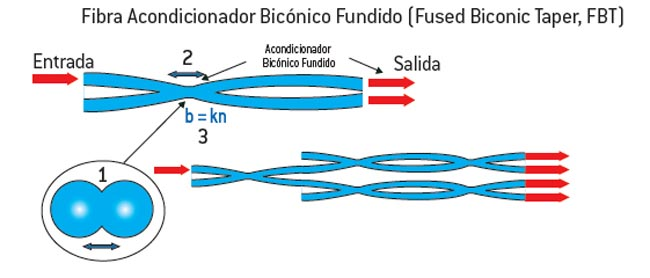
\includegraphics[width=0.86\textwidth]{./img/punto5/Divisor-FBT.jpg}
	\caption{Divisor FBT}
	\label{fig:FBT_splitter}
\end{figure}




 \clearpage
%\\\\\\\\\\\\\\\\\\\\\\\\\\\

%\\\\\\\\\\\\\\\\\\\\\\\\\\\
 \section{Conectores para FTTH}
 \resetallcounters
 Existen tres categorías diferentes de conectores:


\begin{itemize}
\item \textbf{Simplex}, conector con una fibra terminada
\item \textbf{Dúplex}, conector con dos fibras terminadas
\item \textbf{Multifibra}, conector con más de dos fibras (hasta 72)
\end{itemize}


Los conectores simplex son actualmente los más frecuentes para despliegues FTTH. La figura~\figref{fig:Simplex_connectors} muestra los tipos más comunes de conectores simplex:


\begin{figure}[H]
	\centering
	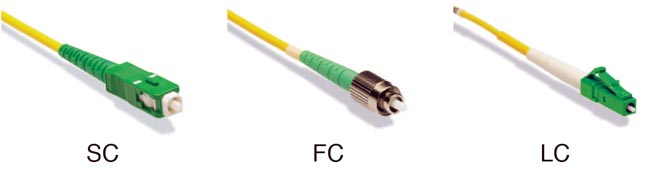
\includegraphics[width=0.80\textwidth]{./img/punto6/Tipos-de-conectores-simplex.jpg}
	\caption{Tipos de conectores simplex}
	\label{fig:Simplex_connectors}
\end{figure}


Otra categoría de conector utilización creciente es el conector multifibra (o MT). Un conector MT individual puede tener desde 4 a 72 fibras. El tipo de conector multifibra utilizado de forma más generalizada en PONs es el tipo MTP. Este conector es utilizado frecuentemente para la confección de latiguillos múltiples de expansión, de especial utilidad en instalaciones de gran densidad de fibras.


\begin{wrapfigure}[10]{l}{0.55\textwidth}
  \begin{center}
   	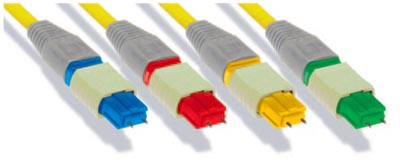
\includegraphics[width=0.55\textwidth]{./img/punto6/Conector-MTP.jpg}	
   	\caption{Conector MTP (fuente US Conec)}
	\label{fig:MTP_connector}
  \end{center}  
\end{wrapfigure}

Cabe indicar, no obstante, que el tipo de conector más frecuente en implantaciones FTTH, por el momento, es el conector de pulido en ángulo (APC), principalmente debido a que la inclinación de 8º en la ferrule proporciona pérdidas de reflexión superiores 60 dB (la pérdida de inserción típica es ≤ 0,5 dB). Los conectores APC pueden identificarse de forma sencilla por su color verde (ver figura~\figref{fig:MTP_connector}).










 \clearpage
%\\\\\\\\\\\\\\\\\\\\\\\\\\\

%\\\\\\\\\\\\\\\\\\\\\\\\\\\
 \section{Equipo de Unidad de Vivienda Colectiva Interior para FTTH}
 \resetallcounters
 En función del tipo de la arquitectura de vivienda colectiva (MDU) que se implantará (ver figura~\figref{fig:MDU_Equipment}), el equipo utilizado puede ser similar al empleado en implantaciones OSP o estar especialmente diseñado para el uso interior (véase la ilustración Equipo de MDU de altura elevada-media). El equipo interior está menos sujeto a condiciones ambientales duras y, por tanto, no requiere el mismo grado de robustez que el equipo de planta exterior (OSP).


\begin{wrapfigure}[25]{l}{0.5\textwidth}
  \begin{center}
   	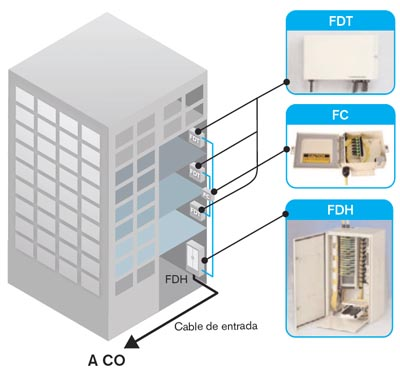
\includegraphics[width=0.5\textwidth]{./img/punto7/Equipo-de-MDU-de-altura-elevada-media.jpg}	
   	\caption{Equipo MDU de altura elevada/media}
	\label{fig:MDU_Equipment}
  \end{center}  
\end{wrapfigure}




Los siguientes elementos se encontrarán normalmente en instalaciones de interior:

Cables de fibra óptica:

\begin{itemize}
\item Los cables de acceso forman el segmento entre la CO y el concentrador de distribución de fibra (FDH) y se encuentran generalmente en el sótano del edificio.
\item Los cables de distribución forman el segmento entre el FDH y el terminal de distribución de fibra (FDT) y se encuentran en cada planta o en el colector de fibra (FC). Los cables de distribución pueden estar formados por una fibra única por puerto divisor o por cables MTP.

\item Los cables de acometida forman el segmento entre el FDT y el ONT y están ubicados en el apartamento. Están generalmente hechos de fibra que es insensible a micro/macrocurvaturas. (Tipo G657)

\end{itemize}

\vfill


\clearpage


Los \textbf{concentradores} de distribución de fibra (FDHs) incluyen:

\begin{itemize}
\item Armarios, cajas de empalmes
\item Divisor(es)
\item Panel(es) de conexiones
\item Elementos de gestión de fibra
\end{itemize}



\textbf{Terminal de distribución} de fibra (FDT):

\begin{itemize}
\item El FDT, ubicado en cada planta, sirve como la conexión entre el FDH y el cable de acometida; puede conectorizarse por fusión (Pigtails) o por conectorización directa (Conectores pre pulidos).
\end{itemize}



\textbf{Colector de fibra} (FC):

\begin{itemize}
\item El FC sirve como un punto de conexión entre el FDH y unos pocos FDTs (ver figura~\figref{fig:Garden_MDU}).
\end{itemize}


\begin{figure}[H]
	\centering
	\includegraphics[width=0.80\textwidth]{./img/punto7/MDU-horizontal-de-estilo-jardín.jpg}
	\caption{MDU horizontal/de estilo jardín}
	\label{fig:Garden_MDU}
\end{figure}


\begin{figure}[H]
	\centering
	\includegraphics[width=0.95\textwidth]{./img/punto7/Enfoques-de-implantación-de-cables-ascendentes-MDU.jpg}
	\caption{Enfoques de implantación de cables ascendentes MDU (aspectos destacados)}
	\label{fig:Ascendant_cables}
\end{figure}




 \clearpage
%\\\\\\\\\\\\\\\\\\\\\\\\\\\



%\\\\\\\\\\\\\\\\\\\\\\\\\\\
% \section{Análisis de resultados obtenidos}
% \resetallcounters
% \input{analisis_resultados.tex}
% \clearpage
%\\\\\\\\\\\\\\\\\\\\\\\\\\\

%\\\\\\\\\\\\\\\\\\\\\\\\\\\
% \section{Diseño y tratamiento acústico para control de reverberación}
% \input{Etapa_2.tex}
% \clearpage
%\\\\\\\\\\\\\\\\\\\\\\\\\\\





%\\\\\\\\\\\\\\\\\\\\\\\\\\\
%Reinicio la cuenta y seteo el estilo de headers y footers.
\pagestyle{bibliostyle}
%\\\\\\\\\\\\\\\\\\\\\\\\\\\



%\\\\\\\\\\\\\\\\\\\\\\\\\\\
\section{Bibliografía}
\resetallcounters

\begin{thebibliography}{9}




\bibitem{Beranek2}
\Needspace*{7\baselineskip}
\emph{Noise and Vibration Control (1\textsuperscript{st} Edition)}\\
Author: Beranek Leo \\
Publisher: Mc. Graw Hill Book Co \\
Copyright: \textcopyright \space 1971, McGraw-Hill\\
ISBN 13: 978-0070048416\\
Website: \weblink{https://www.biblio.com/book/noise-vibration-control-beranek-leo-l/d/1139003044}{https://www.biblio.com/book/noise-vibration-control-beranek-leo-l/d/1139003044}\\






\end{thebibliography}
\cleardoublepage
%\\\\\\\\\\\\\\\\\\\\\\\\\\\

%\\\\\\\\\\\\\\\\\\\\\\\\\\\
%Seteo el stilo de headers y footers.
\pagestyle{allpages}
%\\\\\\\\\\\\\\\\\\\\\\\\\\\

%\appendix
%
%
%\appendixpage
%\addappheadtotoc

%\\\\\\\\\\\\\\\\\\\\\\\\\\\


%\section{Hojas de datos}

%\input{datasheets}

%\clearpage
%\\\\\\\\\\\\\\\\\\\\\\\\\\\





\end{document}
